\chapter{Theoretical Fundamentals}
\section{Introduction to CNNs}

One of the most important elements in CNN models is their hierarchical feature extraction ability. In brief, instead of feeding all raw pixel values directly into a fully connected neural network (FCN), CNNs use convolution operations (also known as the filters) to progressively capture local patterns. The early layers of a CNN learn low-level features like edges, corners, and simple textures. As the network goes deeper, these features can be combined to form higher-level abstractions like eyes, wheels or other shapes, allowing the model to understand more complex structures in the image, in other words, the feature representation gets better in the deeper layers. \\


This feature extraction is achieved by sliding a fixed size filter (usually 3x3) over the input feature map (or input image, in the case of the first layer), multiplying each filter value by the corresponding feature value, and then summing all the results to generate an output value, after going through an activation function, this output becomes the element of the feature map for the next layer. \\
\begin{figure}[H]
 \centering
 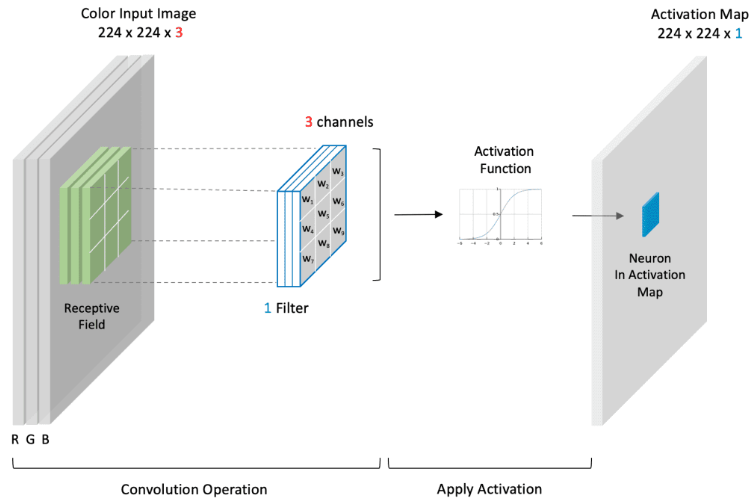
\includegraphics[scale=0.53]{IMAGENES/IMG2-Convolutional_operation.png}
 \captionsetup{font=large}
 \caption {Scheme illustrating the process of a convolutional operation: a 3 x 3 × 3 filter slides over a 224 × 224 × 3 input image, the outputs generated will become the input feature map for the deeper layer. (Image extracted from [2]) }
\end{figure}


In the model architecture, these layers responsible for feature extraction are typically grouped into a module or block called the “backbone”, and it includes all convolution, activation and pooling layers. Once feature extraction is complete, a task-specific block, called the “head”, is applied to produce the final output. For example, for classification tasks, it is common to apply an FCN with a SoftMax activation as the head, as for the classification usually requires a fixed-length output vector with as many elements as classes. Whereas for segmentation tasks, a convolutional layer with a sigmoid activation is usually used, in order to produce a pixel-wise probability mask (2 classes). For multiclass segmentation, a Softmax activation is used across the channel dimension to produce a multi-channel probability map, with one channel per class.\\


Note that “backbone” and “head” are not considered to be universal technical terms, but they are used in some articles and some machine learning frameworks such as PyTorch and Tensorflow to describe the process of transfer learning[3], which is a commonly used technique in model training. In transfer learning, it is common to use a backbone that has been previously trained on a large dataset, it will serve as a general-purpose feature extractor. Then a task-specific head will be added, and the final composite model can be retrained on the target dataset through fine-tuning for the specific task.\\

\section{Model architectures}
One of our objectives in this project is to identify the model architecture that best fits our segmentation task. Therefore, we have selected several CNN-based models and evaluated their performance on our target dataset, which will be discussed in the Model Training section.\\

Next, we will describe shortly each of the model architectures that were evaluated: 
\subsection{2.2.1 U-Net}
\begin{figure}[H]
 \centering
 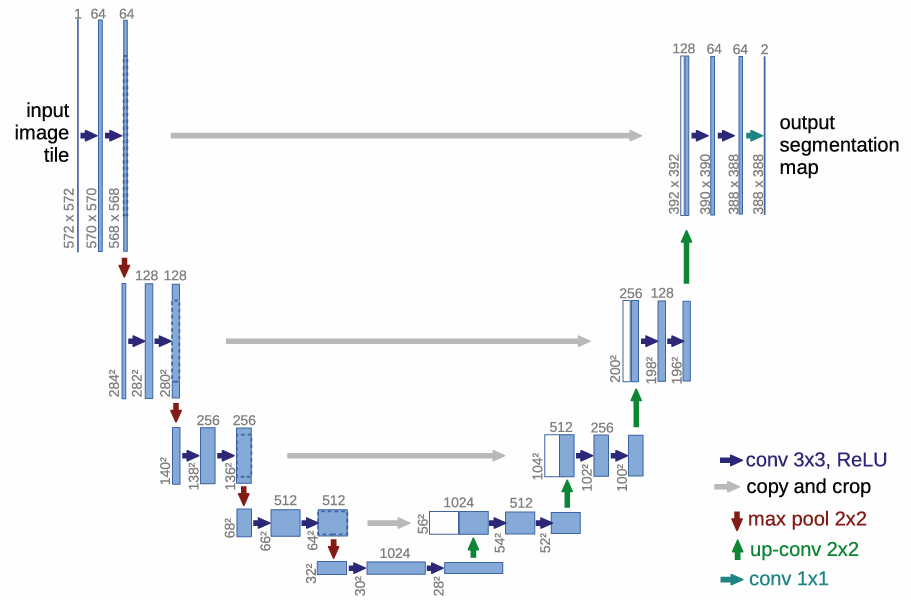
\includegraphics[scale=0.6]{IMAGENES/IMG3-UNet.PNG}
 \captionsetup{font=large}
 \caption {UNet architecture. (Image extracted from [4]) }
\end{figure}

The U-Net is a widely used architecture for segmentation tasks, it was first introduced in (O. Ronneberger, P. Fischer, and T. Brox: "U-net: Convolutional networks for biomedical image segmentation") [4], as the title suggests, the architecture was originally designed for medical image segmentation, in this project we decided to test its performance on our task because, on the one hand, it is simple to implement so it can be a good starting point for experimentation. And on the other hand, we consider that the biostructure identification task is similar to our forest segmentation task since both involve detecting complex patterns and irregular structures. \\


One of the key characteristics of U-Net is its U-shape structure, it consists of a contracting path (encoder) and an expansive path (decoder). The contracting path is generally formed by a series of convolution-pooling blocks (encoder blocks). Each block contains several convolution layers followed by ReLU activations and a max pooling layer. In the contraction process, the max pooling layer progressively reduces the size of the input tensors (input feature maps), forcing the model to learn global context at the cost of losing fine-grained details (which will later be recovered using skip connections). This can also be seen as increasing the receptive field of the neurons (area that each neuron can “see”)[9], since the size of tensors is progressively reducing, a 3x3 filter can cover more information each time . \\


The expansive path is formed by up-convolution blocks (decoder blocks). These blocks enlarge the input tensors back to a higher resolution, and they are linked with their corresponding encoder block through skip connections. In this way, high-resolution tensors from the contracting path will be passed to the expansive path and concatenated with the decoder tensors, helping the model to alleviate the information loss problem and generate a more precise output. \\

\subsection{2.2.2 U-Net++}
\begin{figure}[H]
 \centering
 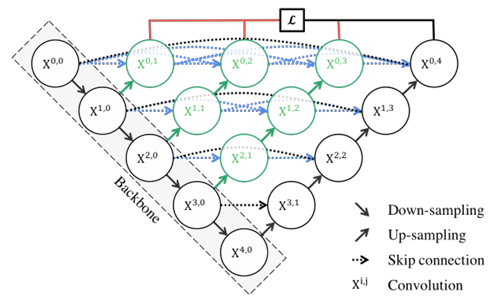
\includegraphics[scale=0.9]{IMAGENES/IMG4-UNetPP.PNG}
 \captionsetup{font=large}
 \caption {UNet++ architecture. (Image extracted from [4]) }
\end{figure}

The original U-Net architecture has been extensively used in many biomedical image segmentation studies due to its remarkable performance, thus, many variants have been designed to further increase segmentation accuracy and robustness.\\


U-Net++ is one of its variants [5], it has a more complex structure than the original U-Net. The main distinction between them resides in the introduction of an additional convolution module (marked as green in the Figure 2.3) that acts as bridges connecting the encoder and decoder. Unlike in the conventional U-Net, where the feature maps of the encoder are passed directly to the decoder, in U-Net++ these maps go through a dense convolution module before being passed to it. The main idea is to bridge the semantic gap between the feature maps of the encoder and decoder prior to fusion, which might make the optimization problem easier [5].\\

\subsection{2.2.3 Attention U-Net}
\begin{figure}[H]
 \centering
 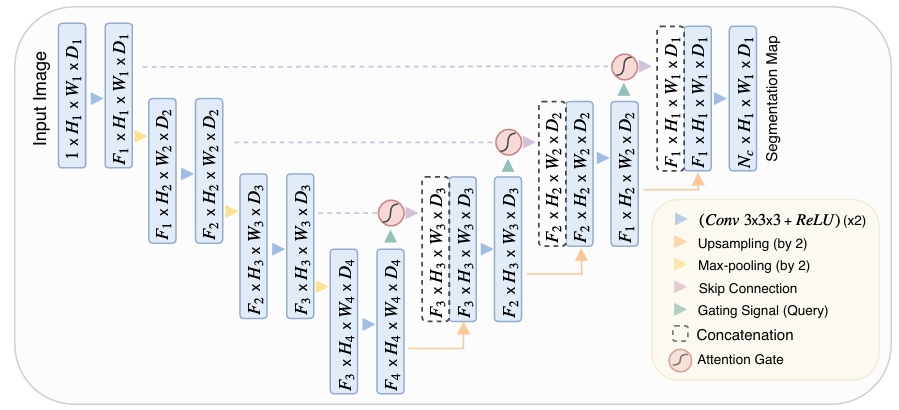
\includegraphics[scale=0.6]{IMAGENES/IMG5-AUNet.PNG}
 \captionsetup{font=large}
 \caption {Attention UNet++ architecture. (Image extracted from [6]) }
\end{figure}

Attention U-Net is another variant of the U-Net architecture that introduces attention mechanisms to improve feature extraction [6]. In this variant, an attention gate is integrated into the skip connections. The feature maps from each encoder block pass through the attention gate before being concatenated with the corresponding decoder tensor.\\

The purpose of the attention gate is to help the model to focus more on target structures of varying shapes and sizes. According to the original ariticle [6], models trained with attention gates are able to suppress irrelevant regions in the input image while emphasizing salient features that are important for the task.\\

The architecture of the attention gate is shown in the following figure: 

\begin{figure}[H]
 \centering
 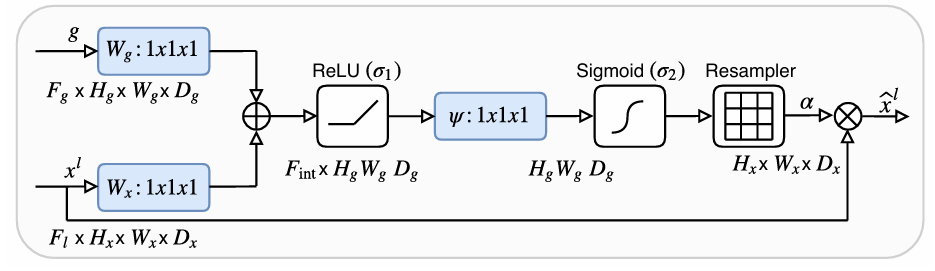
\includegraphics[scale=0.6]{IMAGENES/IMG6-AttentionGate.PNG}
 \captionsetup{font=large}
 \caption {Attention gate architecture. (Image extracted from [6]) }
\end{figure}

The gate mechanism has been well explained in (R. Vinod, “A detailed explanation of the attention u-net.”) [7]. To summarize, the gate receives 2 inputs: the tensor x from the current-level layer, and the tensor g (also known as the signal) from the next-level layer. The tensor g has a smaller dimension but carries better feature representations since it comes from a deeper layer.\\

Both tensors go through a 1x1 convolution (tensor x undergoes an additional max pooling operation to match the spatial dimensions of g). The 2 processed tensors are then summed elementwise, the resulting tensor will have larger values in regions where the weights are aligned, and smaller values where they are not. Then, the tensor will go through a series of convolution-activation blocks and a resampling operation to restore it to the original dimensions of x, obtaining in this way a coefficient tensor called alfa.\\ 

The alfa contains information about the regions-of-interest (regions where the weights are higher) and is used to scale x via elementwise multiplication. This gated tensor is then passed to the decoder blocks through skip connections.\\

\subsection{2.2.4 DeeplabV3+}
\subsection{- Problems in the U-Nets }
The previous architectures are all variants of U-Net, and thus they all share a common limitation: the spatial resolution progressively decreases as the network goes deeper. As explained in the U-Net section, this aims to increase the receptive field of neurons, so that the network can capture global contextual information. This action is usually beneficial for the classification tasks since they require a global understanding of the image. However, it might be harmful for the segmentation tasks, which depend heavily on the spatial information. In other words, as the network goes deeper, it gains more information of “what object is in the image?” but gradually loses information about “where the object is located?”.\\

The key point to alleviate this problem is to increase the receptive field while preserving the spatial resolution. One way to achieve this is by using larger filter sizes (for example, 7x7 instead of 3x3). Since a larger filter can cover a wider area of the input, it allows the network to capture global context without requiring additional spatial reduction. Nevertheless, using a larger filter would also increase the number of parameters and, consequently, the computational complexity. As a solution, the dilated convolutions (also known as atrous convolutions) have been proposed. [10]\\

\subsection{- Dilated convolutions }
\begin{figure}[H]
 \centering
 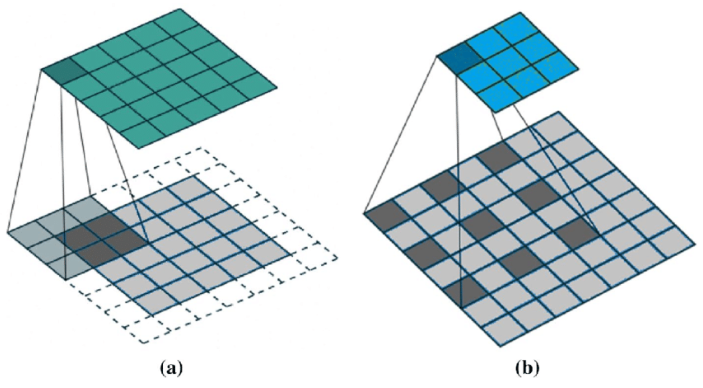
\includegraphics[scale=0.6]{IMAGENES/IMG7.PNG}
 \captionsetup{font=large}
 \caption {a) Traditional convolution. b) Dilated convolution (Atrous convolution) with dilation rate = 2. (Image extracted from [7]) }
\end{figure}

The architecture itself is simple to understand, it can be visualized as a standard convolutional filter with “holes”, created by stretching the original filter so that it can capture a larger portion of the image at once. The number of filter parameters remains unchanged (3x3 parameters), but the filter itself is dilated by inserting gaps between its values, and the pixels corresponding to these gaps are skipped and not taken into account during the elementwise multiplication.\\

The size of the gaps is controlled by a hyperparameter r (also known as the dilation rate). When r=1, the filter reduces to a normal convolutional filter, with no gapes between its elements, and as r increases, the receptive field grows exponentially without increasing the number of parameters. 

\subsection{- ASPP }
\begin{figure}[H]
 \centering
 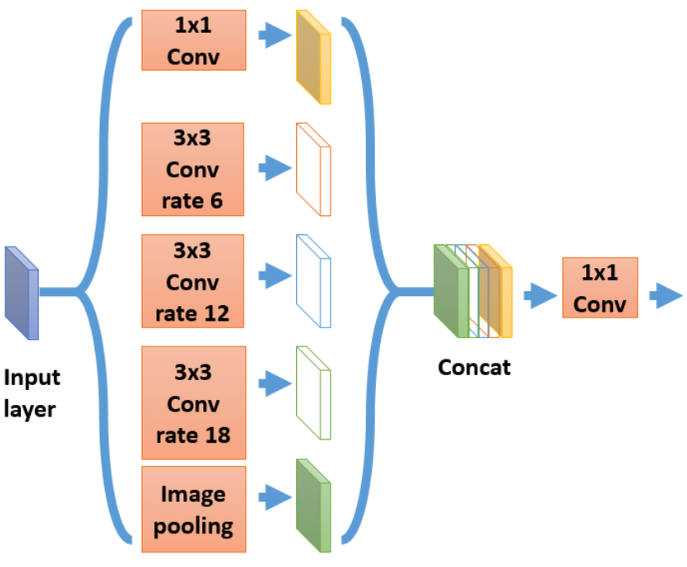
\includegraphics[scale=0.6]{IMAGENES/IMG9-ASPP.PNG}
 \captionsetup{font=large}
 \caption {ASPP module, the module is formed by multiple dilated convolution layers in parallel (Image extracted from [9]) }
\end{figure}
Based on the dilated convolution technique, the Atrous Spatial Pyramid Pooling (ASPP) module has been developed to address another challenge that the U-Nets are facing [14]: An object can appear at different scales in the images. The difficulty of detecting varying sizes objects can usually be alleviated by providing rescaled versions of the same input image to the network. Inspired by this idea, ASPP employs multiple parallel dilated convolutional layers with different dilation rates. Each dilated convolutional layer in ASPP samples the input at a specific resolution to capture the object at that scale, and the outputs of these layers are then concatenated together to produce the final result. 

\subsection{- DeepLabv3+ arquitecture}

One of the most successful models built on the previous techniques is DeepLabV3+ [14], it is the latest successor in the DeepLab series, designed by google researchers for a variety of semantic segmentation tasks. DeepLabV3+ uses a ResNet model as the backbone along with dilated convolutions and ASPP module. The model architecture is shown in the figure below: 

\begin{figure}[H]
 \centering
 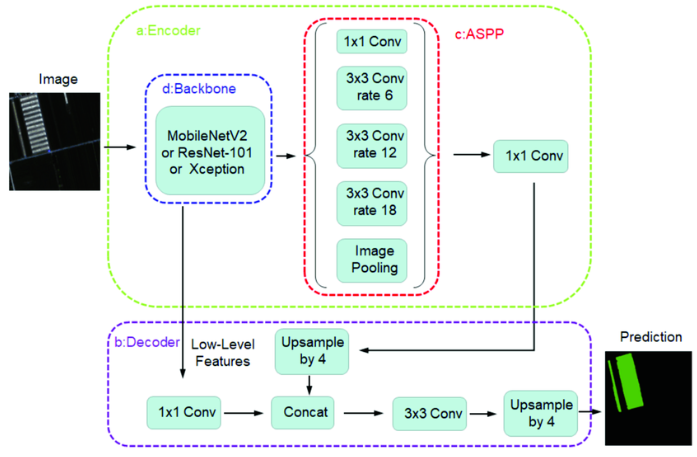
\includegraphics[scale=0.8]{IMAGENES/IMG8-deeplab.PNG}
 \captionsetup{font=large}
 \caption {DeepLabV3+ architecture scheme. The scheme shows an encoder block (a) that contains a ResNet module (d), which acts as backbone for lower-level feature extraction, a ASPP module (c), for multi-scale context extraction. And a decoder block (b), which concatenates the resulting feature maps and up sample them to the original size for final prediction. (Image extracted from [8]) }
\end{figure}

It is important to note that the selection of the backbone is very flexible, ResNet is not a fixed option, for example, it can use a ResNet pretrained on the ImageNet dataset or a MobileNet pretrained on the CoCo dataset [16, 17].  